\begin{enumerate}[\bfseries \mbox{Problema} 1.]

    %-------------------- problema 1
    \item Sean \textbf{\boldmath $x,y \in \mathbb{R}$ con $x,y\neq 0$. Si $\|x\|=\|y\|,$ entonces hallar la medida del ángulo entre $\frac{1}{2}(x+y)$ e $y-x$.\\\\
	Respuesta.-}\; Ya que $x,y\neq 0$ y por el teorema de los cosenos se tiene,
	$$\left\langle \frac{1}{2}(x+y),y-x \right\rangle = \|x\|\|y\|\cos \theta \qquad (1)$$
	Por definición de producto interno y la parte izquierda de $(1)$,
	$$\sum_{i=1}^n \left[\dfrac{1}{2}(x_i+y_i)\cdot (y_i-x_i) \right]= -\dfrac{1}{2}\left(\sum_{i=1}^n x_i^2+\sum_{i=1}^n y_i^2\right) = -\dfrac{1}{2}\left(\langle x,x\rangle + \langle y,y\rangle \right).$$

	Así $(1)$ quedará de la siguiente manera,
	$$\langle x,x\rangle + \langle y,y\rangle = -2\|x\|\|y\|\cos \theta.$$

	Ya que $\|x\|=\|y\|$ y el teorema de cosenos. Entonces,
	$$\|x\|\|x\|\cos \theta + \|y\|\|y|\cos \theta = -2\|x\|\|x\|\cos \theta \quad \Rightarrow \quad \cos \theta \left(3\|x\|\|x\|+\|y\|\|y|\right)=0$$
	Por lo tanto,
	$$\cos \theta = 0 \quad \Rightarrow \quad \theta = \arccos(0) \quad \Rightarrow \quad \theta = \dfrac{\pi}{2}.$$\\
	

    %-------------------- problema 2
    \item \textbf{\boldmath Demuestre que si $x+y$ y $x-y$ son ortogonales, entonces los vectores $x$ e $y$ deben tener la misma longitud.\\\\
	Demostración.-}\; Sea $x.y\in \mathbb{R}^n$. Por definición de ortogonalidad, se tiene
	$$\langle x+y,x-y \rangle=0.$$
	Luego por definición de producto interno,
	$$\begin{array}{rcl}
	    \displaystyle\sum_{i=1}^n \left[(x_i+y_i)(x_i-y_i) \right]&=&0\\\\
	    \displaystyle\sum_{i=1}^n x_i^2 - \displaystyle\sum_{i=1}^n y_i^2&=&0\\\\
	    \langle x,x\rangle - \langle y,y\rangle &=&0\\\\
	    \sqrt{\langle x,x\rangle}&=&\sqrt{\langle y,y\rangle}\\\\
				     \|x\|&=&\|y\|\\
	\end{array}$$
	Ya que la norma mide el tamaño del vector entonces $x$ e $y$  tienen la misma longitud.\\\\


    %-------------------- problema 3
    \item \textbf{\boldmath Sean $x,y\in \mathbb{R}^n$. Demuestre que $\|x+y\|^2=\|x\|^2+\|y\|^2$ si, y solamente si, $x$ e $y$ son ortogonales.\\\\
	Demostración.-}\; Sea $\|x+y\|^2=\|x\|^2+2\langle x,y\rangle + \|y\|^2$. Como $\langle x,y\rangle = 0$, entonces
	$$\|x+y\|^2=\|x\|^2 + \|y\|^2.$$\\


    %-------------------- problema 4
    \item \textbf{\boldmath Demuestre, y dé una interpretación geométrica de, la ley del paralelogramo: Si $x,y\in \mathbb{R}^3$, entonces:
	$$\|x+y\|^2 + \|x-y\|^2=2\left(\|x\|^2+\|y\|^2\right).$$\\
    Demostración.-}\; Ya que $x,y\in \mathbb{R}^3$ y por definición de norma, entonces
    $$\begin{array}{rcl}
	\|x+y\|^2 + \|x-y\|^2 &=& \left(\sqrt{\langle x+y,x+y\rangle}\right)^2+\left(\sqrt{\langle x-y,x-y\rangle}\right)^2\\\\
			      &=&\displaystyle\sum_{i=1}^3 \left[(x_i+y_i)(x_i+y_i)\right]+\sum_{i=1}^3 \left[(x_i-y_i)(x_i-y_i)\right]\\\\
			      &=&\displaystyle\sum_{i=1}^3\left(x_i^2+2x_iy_i+y_i^2\right)+\displaystyle\sum_{i=1}^3\left(x_i^2-2x_iy_i+y_i^2\right)\\\\
			      &=&\displaystyle 2\left(\sum_{i=1}^3x_i^2+\sum_{i=1}^3y_i^2\right) = 2\left(\langle x,x\rangle+\langle y,y\rangle\right)\\\\
			      &=& 2\left[\left(\sqrt{\langle x,x\rangle}\right)^2+\left(\sqrt{\langle y,y\rangle}\right)^2\right]\\\\
			      &=& 2\left(\|x\|^2+\|y\|^2\right).\\\\
    \end{array}$$
    Otra manera de demostrar sería:
    $$\|x+y\|^2 + \|x-y\|^2 = \|x\|^2 + 2\langle x,y\rangle + \|y\|^2 + \|x\|^2 - 2\langle x,y\rangle + \|y\|^2 = 2\left(\|x\|^2+\|y\|^2 \right).$$\\


    %-------------------- problema 5
    \item \textbf{\boldmath Calcule el ángulo formado por los diagonales de dos caras consecutivas de un cubo de arista igual a $a$.\\\\
	Demostración.-}\; Ya que se tiene un cubo. Entonces,\\
	\begin{center}
	    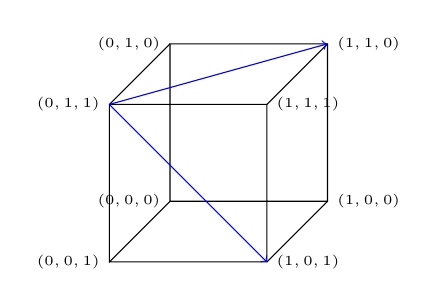
\begin{tikzpicture}[scale=2]
		\draw[](0,0,0)node[left]{\tiny$(0,0,0)$}--(0,1,0)node[left]{\tiny$(0,1,0)$}--(1,1,0)node[right]{\tiny$(1,1,0)$}--(1,0,0)node[right]{\tiny$(1,0,0)$}--(0,0,0)--(0,0,1)node[left]{\tiny$(0,0,1)$}--(0,1,1)node[left]{\tiny$(0,1,1)$}--(1,1,1)node[right]{\tiny$(1,1,1)$}--(1,0,1)node[right]{\tiny$(1,0,1)$}--(0,0,1);
		\draw[](1,1,1)--(1,1,0);
		\draw[](0,1,1)--(0,1,0);
		\draw[](1,0,1)--(1,0,0);
		\draw[blue,->](0,1,1)--(1,0,1);
		\draw[blue,->](0,1,1)--(1,1,0);
	    \end{tikzpicture}
    \end{center}
    Luego se tiene al vector $x=(1,0,1)-(0,1,1)=(1,-1,0)$ y $y = (1,1,0)-(0,1,1)=(1,0,-1)$, por lo tanto el angulo será:
    $$\begin{array}{rcl}
	\cos \theta &=& \dfrac{\langle (1,-1,0),(1,0,-1)\rangle}{\|(1,-1,0)\|\|(1,0,-1)\|}\\\\ 
		    &=& \dfrac{1\cdot 1 + (-1)\cdot 0 + 0\cdot (-1)}{\sqrt{1^2+(-1)^2+0^2}\cdot \sqrt{1^2+0^2+(-1)^2}}\\\\
		    &=&\dfrac{1}{\left(\sqrt{2}\right)^2}=\dfrac{1}{2}.\\\\
    \end{array}$$
    Por lo tanto,
    $$\theta = \dfrac{\pi}{3}$$\\

    %-------------------- problema 6
    \item \textbf{\boldmath Demuestre que todo triángulo inscrito en una semicircunferencia es recto.\\\\
	Demostración.-}\;

    %-------------------- problema 7
    \item \textbf{\boldmath Demuestre que uniendo los puntos medios de los lados de un cuadrilátero se obtiene un paralelogramo.\\\\
	Demostración.-}\;

    %-------------------- problema 8
    \item \textbf{\boldmath Demuestre que el punto medio de la hipotenusa de un triángulo rectángulo es equidistante de los tres vertices.\\\\
	Demostración.-}\;

    %-------------------- problema 9
    \item \textbf{\boldmath Demuestre que el segmento que une los puntos medios de dos lados de un triángulo es paralelo al tercer lado y tiene la mitad de su longitud.\\\\
	Demostración.-}\;

    %-------------------- problema 10
    \item \textbf{\boldmath Pruebe la ley de senos utilizando vectores.\\\\
	Demostración.-}\; 

    %-------------------- problema 11
    \item \textbf{\boldmath Muestre que las medianas de un triángulo se cortan en un punto a un tercio de cada mediana.\\\\
	Demostración.-}\;

    %-------------------- problema 12
    \item \textbf{\boldmath Demuestre que las diagonales de un rombo son ortogonales entre si.\\\\
	Demostración.-}\;

    %-------------------- problema 13
    \item \textbf{\boldmath Si $x,y,z \in \mathbb{R},$ entonces demostrar que:
	$$x\times (y \times z) = \langle x,z\rangle y - \langle x,y\rangle z.$$\\
	Demostración.-}\;

    %-------------------- problema 14
    \item \textbf{\boldmath Sean $x,y\in \mathbb{R}^3$ con $x,y\neq 0.$ Si $\dfrac{\|x\times y\|}{\|x\|^3}=3,$ entonces hallar $\dfrac{\| \langle x,x\rangle y - \langle x,y\rangle x \|}{\|x\|^4}$.\\\\
	Demostración.-}\;

    %-------------------- problema 15
    \item \textbf{\boldmath Si $x,y\in \mathbb{R}^3$, entonces demostrar que:
    $$\|x\times y\|^2 = \|x\|^2 \|y\|^2 - \langle x,y \rangle^2.$$\\
	Demostración.-}\;

    %-------------------- problema 16
    \item \textbf{\boldmath Si $x,y,z \in \mathbb{R}^3,$ entonces demostrar que:
    $$x\times (y\times z) + y \times (z\times x)+z\times(x\times y)=0.$$\\
	Demostración.-}\;


\end{enumerate}
